\chapter{Einleitung}\label{Einleitung}
\section{Einführung}
In dieser Bachelorarbeit werden die Themen \emph{Klassifikation} und \emph{Clustering} in Bezug auf heuristische Methoden behandelt. In der heutigen Welt sind große Datenmengen an der Tagesordnung. Die Hardware ist zwar leistungsfähig genug, kann aber große Datensätze nicht auf einmal verarbeiten, da die zeitliche Datendurchsatzrate zu gering ist. Daher ist es entscheidend große Datenmengen in kleinere Einheiten mit Hilfe von Klassifikation und Clustering überzuführen. Der Begriff \textit{Big Data} bestimmt die Welt der Analyse und der Verarbeitung von Informationen, welche meist als mehrdimensionale Daten beschrieben werden können. Daher ist es wichtig geeignete Algorithmen und Verfahren zu finden, welche große Datenmengen in anwendbare Einheiten einteilen.\\Das Ziel der Analyse von eingeteilten Daten ist es eine verständliche und interpretierbare Konzeption zu erreichen, welche auf einem geeigneten Modell basiert. Dieses Modell kann nur auf der Basis von eingeteilten Daten funktionieren, da es sonst zu komplex wird. Das Clustering und die Klassifikation machen diese Vorgangsweise erst möglich. Sie sind daher ein zentraler Bestandteil bei der Analyse von Daten und in der Heuristik und in der Statistik nicht mehr wegzudenken.  
\section{Aufgabenstellung}
In der Klassifikation geht es darum Samples in verschiedene Klassen einzuteilen. Beim Clustering dagegen geht es darum Gruppen von Datenpunkten zu identifizieren. Ist es sinnvoll Daten vor dem Anwenden von Klassifikationsalgorithmen zu gruppieren, also Clustering und Klassifikation zu kombinieren. Lässt sich so die Prognosegenauigkeit erhöhen? Ziel dieser Arbeit ist es, Antworten auf diese Fragen zu finden; Frameworks wie das HeuristicLab und WEKA sowie international bekannte Benchmark-Datensätze können für die entsprechenden Tests verwendet werden.


\section{Terminologien und Begrifflichkeiten}
\begin{itemize}
	\item \textbf{Heuristik:}\\ Aus dem Griechischen heuriskein = finden, entdecken, bezeichnet eine Erfinderkunst. Heuristik ist die Lehre von verschiedenen Verfahren zum Lösen von Problemen, welche nicht mit mathematischen Algorithmen bzw. Formeln gelöst werden können.
\item \textbf{Datensatz:}\\ Ein Datensatz ist die Zusammenfassung von Daten, die in einer direkten Beziehung zueinander stehen oder gemeinsame Merkmale haben. Daten, die in einem Sinnzusammenhang stehen, können dabei in einem Ordnungssystem zusammengefasst sein.
\item \textbf{Wahrscheinlichkeit:}\\ Die Wahrscheinlichkeit ist ein Maß zur Quantifizierung der Sicherheit bzw. Unsicherheit des Eintretens eines bestimmten Ereignisses im Rahmen eines Zufallsexperiments
\item \textbf{Algorithmus:}\\Ein Algorithmus ist eine eindeutige, ausführbare Folge von Anweisungen endlicher Länge zur Lösung eines Problems. Ein Algorithmus besteht aus einem Deklarationsteil und einem Anweisungsteil.
\item \textbf{Sample (Sampling):}\\Teilmenge einer Grundgesamtheit, die für eine Untersuchung ausgewählt wird.
\item \textbf{Satz von Bayes:}\\Der Satz von Bayes ist ein mathematischer Satz aus der Wahrscheinlichkeitstheorie, der die Berechnung bedingter Wahrscheinlichkeiten beschreibt. Formel: \[P(A|B)=\frac{P(A)\cdot P(B|A)}{P(B)}=\frac{P(A\cap B)}{P(B)}\]
\item \textbf{Test:}\\ Tests sind Methoden, mit denen eine Entscheidung über die Beibehaltung oder Zurückweisung einer Nullhypothese \(H_0\) mithilfe eines Stichprobenbefundes getroffen wird.
\item \textbf{Graph:}\\Ein Graph ist in der Graphentheorie eine abstrakte Struktur, die eine Menge von Objekten zusammen mit den zwischen diesen Objekten bestehenden Verbindungen repräsentiert. Die mathematischen Abstraktionen der Objekte werden dabei Knoten des Graphen genannt. Die paarweisen Verbindungen zwischen Knoten stellen Kanten dar.
\item \textbf{Daten:}
	\begin{itemize}
		\item numerisch:\\Daten, die  mit Ziffern und zusätzlichen Sonderzeichen dargestellt werden.
		\item nicht-numerisch:\\Daten, die aus Buchstaben und Ziffern zusammengesetzt sind.
	\end{itemize}
	\item \textbf{Zeitreihe:}\\Ein Zeitreihe ist eine Serie von Messungen, Beobachtungen und Aufzeichnungen von Variablen an aufeinanderfolgenden Zeitpunkten. Zeitreihen ermöglichen eine strukturierte Darstellung von Daten. Eine visuelle Darstellung entspricht einer Kurve, die sich mit der Zeit entwickelt.
	\item \textbf{Dimension:}\\  Der Begriff Dimension bezeichnet im Allgemeinen lediglich ein unabhängiges Merkmal eines Datensatzes. Dimensionen haben mit den Daten selbst gar keine echte Verwandtschaft, sondern stellen meist ein unabhängiges Gedankenkonstrukt dar, das Analogien zum Datensatz herstellt, um es berechenbar oder messbar zu machen.
\item \textbf{Distanzmaß:}\\ Als Distanzmaß wird ein Maß bezeichnet, wenn es die Unähnlichkeit zwischen zwei Objekten misst. Es besitzt die Eigenschaft, dass es mit zunehmender Unterschiedlichkeit zweier Objekte ansteigt.
\item \textbf{Kostenfunktion:}\\ Als Kostenfunktion wird jene Funktion beschrieben, welche bestimmt wie komplex und aufwendig ein Algorithmus oder Verfahren ist. Meist wird diese Funktion mit der O-Notation gleich gesetzt, welche vor allen in der Laufzeitmessung angewandt wird.
\item \textbf{Lagemaße:}
	\begin{itemize}
		\item Mittelwert:\\ Der Mittelwert beschreibt den statistischen Durchschnittswert und wird auch arithmetisches Mittel genannt. 
		\item Median:\\Der Wert, der genau in der Mitte einer Datenverteilung liegt, nennt sich Median oder Zentralwert. Die eine Hälfte aller Daten ist immer kleiner, die andere größer als der Median. 
		\item Modus:\\Der Modus gibt an, welche Merkmalsausprägung in einem Datensatz am häufigsten vorkommt. 
\end{itemize}
\item \textbf{Heatmap:}\\
Eine Heatmap  ist ein Diagramm zur Visualisierung von Daten, deren abhängige Werte einer zweidimensionalen Definitionsmenge als Farben repräsentiert werden. Sie dient dazu, in einer großen Datenmenge intuitiv und schnell besonders markante Werte zu erfassen.
\begin{figure}[H]
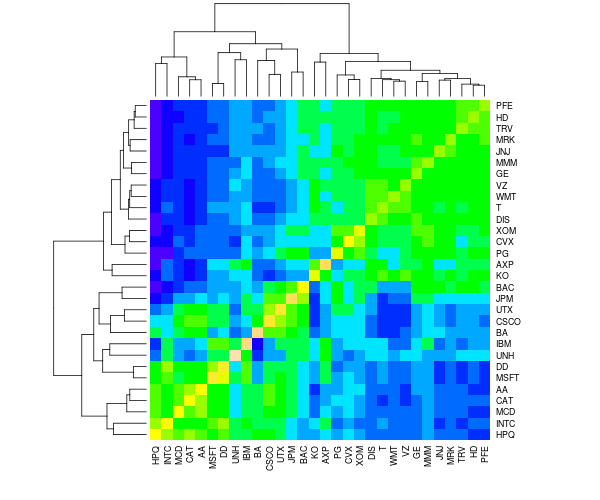
\includegraphics[width=\textwidth]{Heatmap.png}
\caption{heatmap}
\label{}
\end{figure}
\item \textbf{Cluster:}\\
Als Cluster bezeichnet man in der Informatik und Statistik eine Gruppe von Datenobjekten mit ähnlichen Eigenschaften.
\item \textbf{Link Arten:}
\begin{itemize}
		\item Single-Link:\\ Beschreibt die kleinste Entfernung von den Clustern und wird auch als nächster Nachbar bezeichnet.
		\item Average-Link:\\Beschreibt die mittlere Distanz von Clustern zueinander
		\item Complete-Link:\\ Beschreibt die maximale Entfernung von Clustern zueinander.
\end{itemize}
\end{itemize}
